\documentclass[10pt,oneside]{mwbk}

% ustawienia kodowania pliku i języka
\usepackage[T1]{polski}
\usepackage[utf8]{inputenc}

\usepackage{indentfirst}
\usepackage{graphicx}


% czcionka Times
\usepackage{times}

% odstępy na 1.5 (pomimo, iż linespread jest na 1.3
\linespread{1.3}

% dzielenie wyrazów – większe odstępy, mniej dzielenia
\hyphenpenalty=5000
\tolerance=5000

%import z pliku csv
\usepackage{csvsimple}

%strona tytułowa
\renewcommand {\maketitle}{
\begin {titlepage}
\begin {center}
	\LARGE
	\textbf {PROJEKTOWANIE ALGORYTMOW I METODY SZTUCZNEJ INTELIGENCJI}
	\newline
	\newline
	\textit {SPRAWOZDANIE Z  LABORATORIUM}
	\textbf{ Quicksort - wpływ metody wyboru piwotu na czas sortowania}
	\newline
	\begin{table}
	\begin{center}
	\begin{tabular}{rl}
	IMIĘ I NAZWISKO & Mariusz Dajczak \\
	NR INDEKSU & 200403 \\	
	TERMIN & czwartek 10:00-12:35 \\
	DATA  & 27.03.2014 \\
	\end{tabular}

	\end{center}
	\end{table}
\end {center}
\end {titlepage}}

\renewcommand*\thesection{\arabic{section}} % zmiana numeracji sekcji 0.X -> X
\begin{document}
\maketitle
\section{Wstęp}
	

	\indent Algorytm sortowania szybkiego jest uważany za najszybszy jesli chodzi o dane losowe. Oparty jest na metodzie dziel i zwyciężaj. Polega to na tym, że zbiór danych zostaje podzielony na dwa podzbiory i każdy z nich jest sortowany niezależnie.
	W średnim przypadku jego złożoność obliczeniowa wynosi $nlogn$ , natomiast w najgorszym $n^{2}$.\\
	
	\indent Quicksort w podstawowej wersji za piwot obiera pierwszy lub ostatni element zbioru. Taki sposób działania jest poprawny i powszechnie stosowany, jednak aby zminimalizować prawdopodobieństwo przypadku pesymistycznego można losowwo wybierać piwot. Dzięki temu trickowi szansa na wystąpienie najgorszego scenariusza jest statystycznie znacznie mniejsza.\\
	\\
	\indent Celem tego ćwiczenia jest zbadanie jak zmieni się czas wykonania sortowania obydwoma rodzajami sortowania szybkiego w przypadku średnim oraz pesymistycznym.
	
\section {Wyniki symulacji}
	\textbf{CZASY SORTOWANIA W PESYMISTYCZNYM PRZYPADKU}
	\\

	\begin{table}[!h]
	\centering
	\begin{tabular}{| l | l | l |}
	\hline
	Rozmiar & Powtórzenia & Czas         \\ \hline
	10&5&30.4\\ \hline
100&5&305\\ \hline
1000&5&3820.2.2\\ \hline
10000&5&36122.6\\ \hline
100000&5&594501\\ \hline
1000000&5&5.82638e+006\\ \hline
10000000&5&6.80988e+007\\ \hline
	\end{tabular}
	\caption{Czas sortowania podstawowym Quicksortem}
	\end{table}
	
	
	\begin{table}[!h]
	\centering
	\begin{tabular}{| l | l | l |}
	\hline
		Rozmiar & Powtórzenia & Czas         \\ \hline
10&5&29.4\\ \hline
100&5&244.2\\ \hline
1000&5&2007\\ \hline
10000&5&26304.6\\ \hline
100000&5&279041\\ \hline
1000000&5&3.83514e+006\\ \hline
10000000&5&4.11167e+007\\ \hline
	\end{tabular}
		\caption{Czas sortowania Quicksortem z losowym doborem piwotu}
	\end{table}
	
	
	\newpage
	\textbf{CZASY SORTOWANIA W ŚREDNIM PRZYPADKU}
	\\
	
	\begin{table}[!h]
	\centering
	\begin{tabular}{| l | l | l |}
	\hline
	Rozmiar & Powtórzenia & Czas         \\ \hline
10&10&38.8\\ \hline 
100&10&571.2\\ \hline
1000&10&6624.1\\ \hline
10000&10&77038.7\\ \hline
100000&10&564664\\ \hline
1000000&10&8.1971e+006\\ \hline
10000000&10&7.36563e+007\\ \hline
	\end{tabular}
		\caption{Czas sortowania podstawowym Quicksortem}
	\end{table}
	

	\begin{table}[!h]
	\centering
	\begin{tabular}{| l | l | l |}
	\hline
		Rozmiar & Powtórzenia & Czas         \\ \hline
10&5&51.4\\ \hline
100&5&459.6\\ \hline
1000&5&5304.2\\ \hline
10000&5&24957.6\\ \hline
100000&5&286556\\ \hline
1000000&5&3.79507e+006\\ \hline
10000000&5&4.14374e+007\\ \hline
	\end{tabular}
	\caption{Czas sortowania Quicksortem z losowym doborem piwotu}
	\end{table}

\section {Wykresy}
	\begin{figure}[!ht]
	\centering
	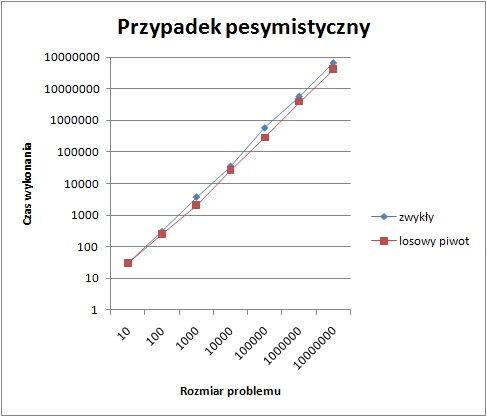
\includegraphics[scale=0.7]{rys/pesymistycznie.jpg}
	\caption{ Złożoność obliczeniowa sortowania w przypadku pesymistycznym}
	\end{figure}
	
	\begin{figure}[!h]
	\centering
	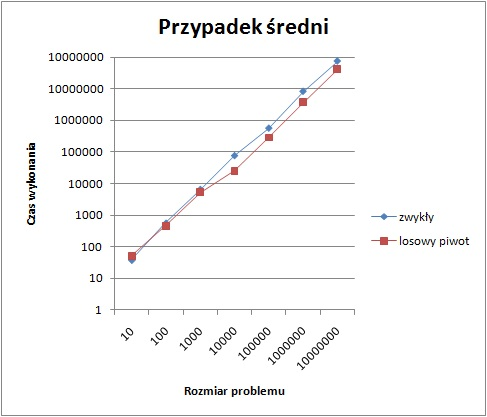
\includegraphics[scale=0.7]{rys/srednio.jpg}
	\caption{ Złożoność obliczeniowa sortowania w przypadku srednim}
	\end{figure}
\newpage
\section {Wnioski}
\indent Po przeprowadzeniu symulacji da się zauważyć pewną różnicę między czasem wykonania obu metod.
W przypadku pesymistycznym losowe wybieranie piwotu jest szybsze dla kazdego rozmiaru problemu. Wynik jest zgodny z oczekiwaniami. 
\indent W średnim przypadku losowanie piwotu również sprawia, że czas wykonania jest krótszy. Wynika to z faktu, że losowe wybieranie piwotu sprawia, iż statystycznie rzecz biorąc mamy większe szanse na uzyskanie przypadku korzystniejszego dla sortowania szybkiego. \\
\indent Zastosowanie tej metody wyboru piwotu usprawnia działanie sortowania szybkiego i sprawia, że jest ono jeszcze bardziej użyteczne. 
\end{document}